\documentclass[a4paper, 10pt]{article}
\usepackage{../../CEDT-Homework-style}

\usepackage{amsmath}
\allowdisplaybreaks

\setlength{\headheight}{14.49998pt}

\begin{document}
\subject[2110203 - Computer Engineering Mathematics II]
\hwtitle{Signal 2}{}{Week 2}{6733172621 Patthadon Phengpinij}{ChatGPT (for\,\LaTeX\,styling and grammar checking)}


% ================================================================================ %
\section{Convolution}
% ================================================================================ %



% ================================================================================ %
%                                    Problem 01                                    %
% ================================================================================ %
\begin{problem}
Evaluate the convolution of the following signals
\end{problem}

% === Problem 1.1. === %
\begin{subproblems}[start=1]
    \item \( \textrm{rect} \paren{ \frac{t-a}{a} } * \delta (t-b) \)
\end{subproblems}

\begin{solution}
From the sifting property of the delta function, we have:
\[ f(t) * \delta(t - b) = f(t - b) \]

Applying this property to our problem, we get:
\[ \textrm{rect} \paren{ \frac{t - a}{a} } * \delta(t - b) = \textrm{rect} \paren{ \frac{(t - b) - a}{a} } = \textrm{rect} \paren{ \frac{t - (a + b)}{a} } \]

Thus, the result of the convolution is:
\[ \boxed{ \textrm{rect} \paren{ \frac{t - (a + b)}{a} } } \]

Using Python to verify this result, we can implement the convolution and plot the results.
The plot of the signal is shown below:
\begin{center}
    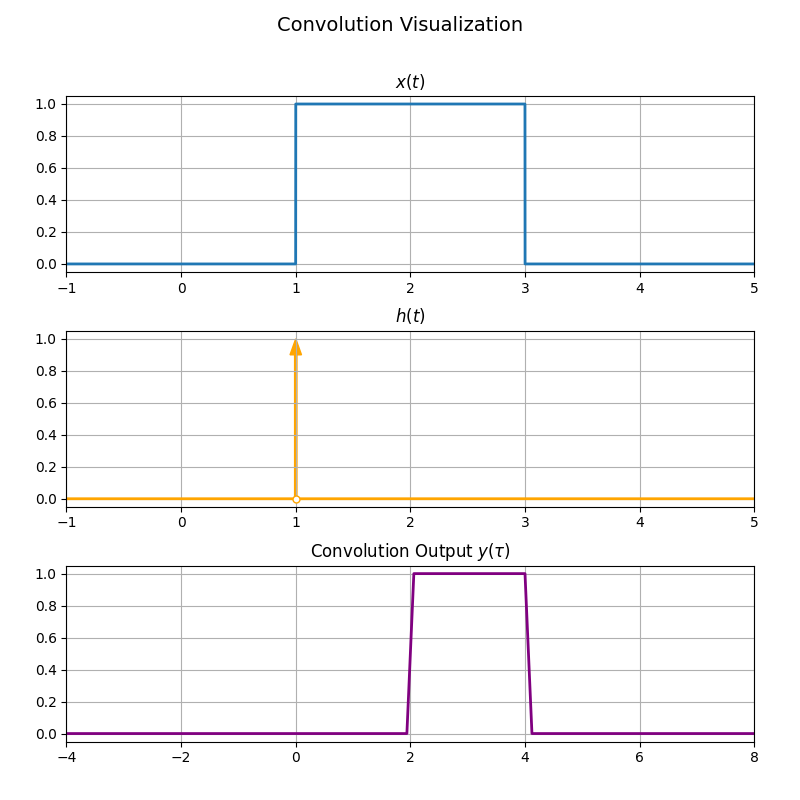
\includegraphics[width=0.7\textwidth]{images/problem_1_1_snapshot.png}
\end{center}
\end{solution}
% ==================== %

\newpage

% === Problem 1.2. === %
\begin{subproblems}[resume]
    \item \( \textrm{rect} \paren{ \frac{t}{a} } * \textrm{rect} \paren{ \frac{t}{a} } \)
\end{subproblems}

\begin{solution}
To evaluate the convolution of two rectangular functions, we start with the definition of the rectangular function:
\[ \textrm{rect} \paren{ \frac{t}{a} } = \begin{cases} 1 & \text{if } |t| \leq \frac{a}{2} \\ 0 & \text{otherwise} \end{cases} \]

The convolution of two functions \( f(t) \) and \( g(t) \) is defined as:
\[ (f * g)(t) = \int_{-\infty}^{\infty} f(\tau) g(t - \tau) \, d\tau \]

Applying this to our rectangular functions, we have:
\[
\begin{aligned}
    ( \textrm{rect} \paren{ \frac{t}{a} } * \textrm{rect} \paren{ \frac{t}{a} } )(t) &= \int_{-\infty}^{\infty} \textrm{rect} \paren{ \frac{\tau}{a} } \textrm{rect} \paren{ \frac{t - \tau}{a} } \, d\tau \\
    &= \int_{-\frac{a}{2}}^{\frac{a}{2}} \textrm{rect} \paren{ \frac{t - \tau}{a} } \, d\tau \\
    &= \int_{\max(-\frac{a}{2}, t - \frac{a}{2})}^{\min(\frac{a}{2}, t + \frac{a}{2})} 1 \, d\tau \\
    ( \textrm{rect} \paren{ \frac{t}{a} } * \textrm{rect} \paren{ \frac{t}{a} } )(t) &= \min\left(\frac{a}{2}, t + \frac{a}{2}\right) - \max\left(-\frac{a}{2}, t - \frac{a}{2}\right)
\end{aligned}
\]

Evaluating the limits, we find that the result is a triangular function:
\[ \boxed{ \textrm{rect} \paren{ \frac{t}{a} } * \textrm{rect} \paren{ \frac{t}{a} } = \begin{cases} 
    0 & |t| > a \\
    t + a & -a \leq t < 0 \\
    a - t & 0 \leq t \leq a
\end{cases} } \]

Using Python to verify this result, we can implement the convolution and plot the results.
The plot of the signal is shown below:
\begin{center}
    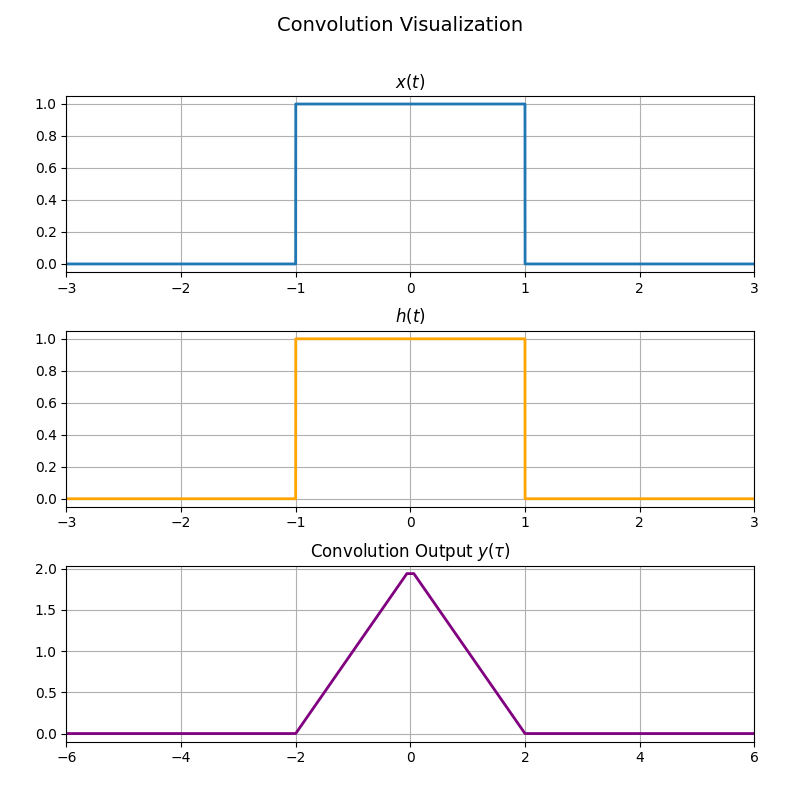
\includegraphics[width=0.7\textwidth]{images/problem_1_2_snapshot.png}
\end{center}
\end{solution}
% ==================== %

\newpage

% === Problem 1.3. === %
\begin{subproblems}[resume]
    \item \( t[u(t)-u(t-1)]*u(t) \)
\end{subproblems}

\begin{solution}
First, we define the functions involved in the convolution:
\[ x(t) = t[u(t) - u(t-1)] = \begin{cases} 0 & t < 0 \\ t & 0 \leq t < 1 \\ 0 & t \geq 1 \end{cases} \]
\[ u(t) = \begin{cases} 0 & t < 0 \\ 1 & t \geq 0 \end{cases} \]

The convolution \( y(t) = x(t) * u(t) \) is given by:
\[ y(t) = \int_{-\infty}^{\infty} x(\tau) u(t - \tau) \, d\tau \]

Evaluating the convolution integral, we find:
\begin{align*}
    y(t) &= \int_{0}^{1} \tau \cdot u(t - \tau) \, d\tau \\
    y(t) &= \int_{0}^{\min(t, 1)} \tau \, d\tau
\end{align*}

Thus,
\[ \boxed{
y(t) = \begin{cases} 
    0 & t < 0 \\
    \frac{t^2}{2} & 0 \leq t < 1 \\
    \frac{1}{2} & t \geq 1
\end{cases}
} \]

Using Python to verify this result, we can implement the convolution and plot the results.
The plot of the signal is shown below:
\begin{center}
    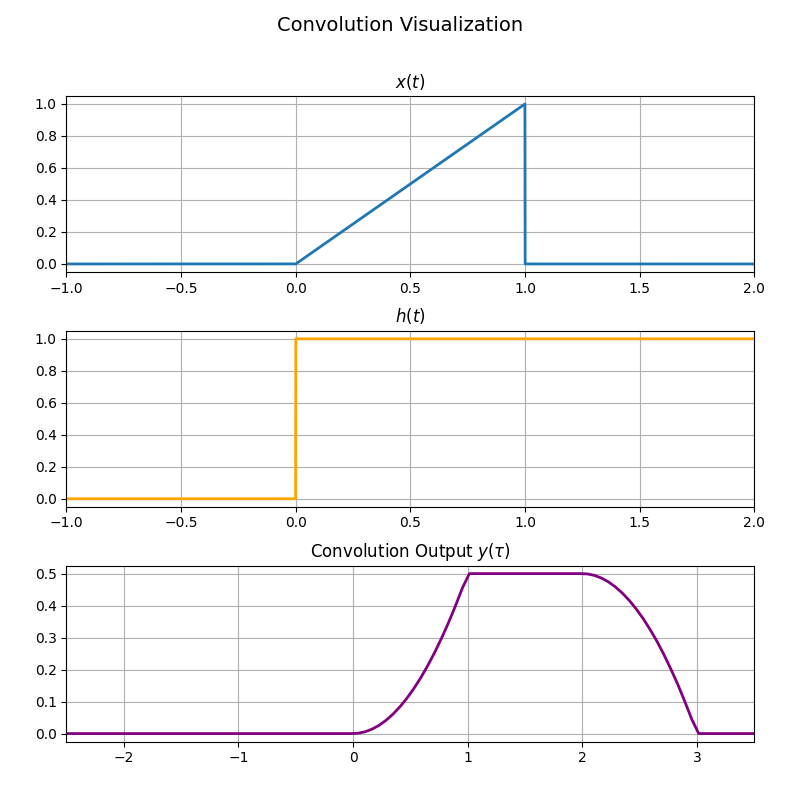
\includegraphics[width=0.7\textwidth]{images/problem_1_3_snapshot.png}
\end{center}
\end{solution}
% ==================== %
% ================================================================================ %

\newpage

% ================================================================================ %
%                                    Problem 02                                    %
% ================================================================================ %
\begin{problem}
Determine the convolution \( y(t) = h(t)*x(t) \) using Graphical Interpretation of the pairs of the signals shown
\end{problem}

\begin{solution}
The convolution \( y(t) = h(t) * x(t) \) can be determined graphically by following these steps:
\begin{enumerate}
    \item Flip one of the signals, typically \( h(t) \), to get \( h(-\tau) \).
    \item Shift the flipped signal by \( t \) to get \( h(t - \tau) \).
    \item For each value of \( t \), calculate the area of overlap between \( x(\tau) \) and \( h(t - \tau) \).
    \item The value of the convolution \( y(t) \) at each \( t \) is the area of overlap calculated in the previous step.
\end{enumerate}
Using Python to visualize and compute the convolution graphically, we can create an animation that demonstrates the convolution process step-by-step.

\vspace{3mm}

The resulting convolution \( y(t) \) is shown in the gif files in \href{https://github.com/patthadon-p/CEDT-2110203-CEM-II/tree/main/signal/homework-2/images}{my GitHub repository} for this homework.
\end{solution}


% === Problem 2.1. === %
\begin{tosubmit}
\begin{subproblems}[start=1]
    \item \submitsolution
\end{subproblems}

Using Python to visualize and compute the convolution graphically,
we can create an animation that demonstrates the convolution process step-by-step
as shown in the gif files in \href{https://github.com/patthadon-p/CEDT-2110203-CEM-II/blob/main/signal/homework-2/images/problem_2_1.gif}{Problem 2.1 Animation}.

\vspace{3mm}

The plot of the signal is shown below:
\begin{center}
    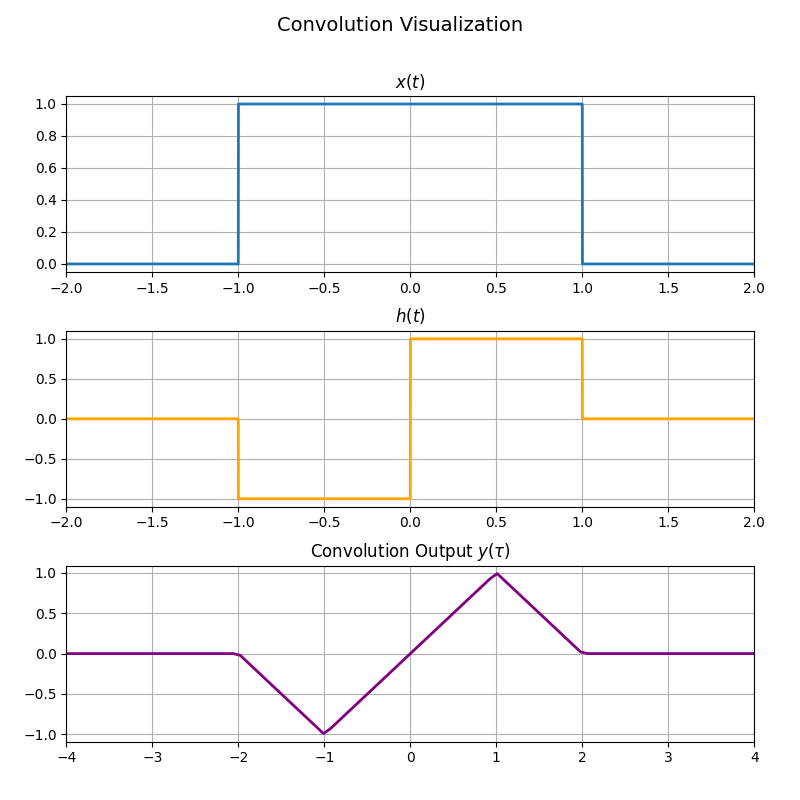
\includegraphics[width=0.75\textwidth]{images/problem_2_1_snapshot.png}
\end{center}
\end{tosubmit}
% ==================== %

\newpage 

% === Problem 2.2. === %
\begin{subproblems}[start=2]
    \item
\end{subproblems}

\begin{solution}
    Using Python to visualize and compute the convolution graphically,
    we can create an animation that demonstrates the convolution process step-by-step
    as shown in the gif files in \href{https://github.com/patthadon-p/CEDT-2110203-CEM-II/blob/main/signal/homework-2/images/problem_2_2.gif}{Problem 2.2 Animation}.
    
    \vspace{3mm}
    
    The plot of the signal is shown below:
    \begin{center}
        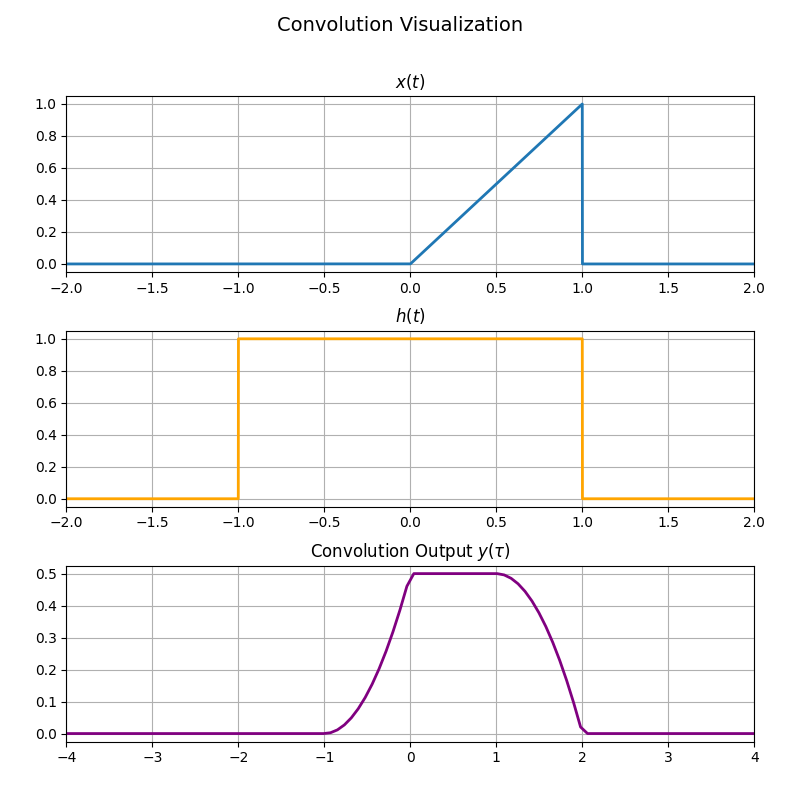
\includegraphics[width=0.75\textwidth]{images/problem_2_2_snapshot.png}
    \end{center}
\end{solution}
% ==================== %

\newpage

% === Problem 2.3. === %
\begin{tosubmit}
\begin{subproblems}[start=3]
    \item \submitsolution
\end{subproblems}

Using Python to visualize and compute the convolution graphically,
we can create an animation that demonstrates the convolution process step-by-step
as shown in the gif files in \href{https://github.com/patthadon-p/CEDT-2110203-CEM-II/blob/main/signal/homework-2/images/problem_2_3.gif}{Problem 2.3 Animation}.

\vspace{3mm}

The plot of the signal is shown below:
\begin{center}
    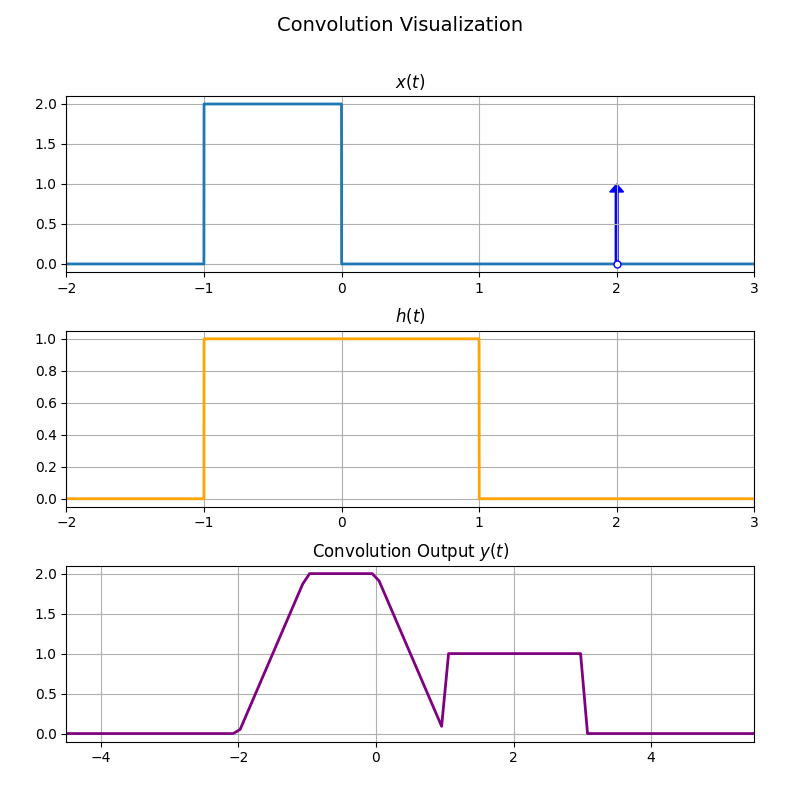
\includegraphics[width=0.75\textwidth]{images/problem_2_3_snapshot.png}
\end{center}
\end{tosubmit}
% ==================== %

\newpage 

% === Problem 2.4. === %
\begin{subproblems}[start=4]
    \item
\end{subproblems}

\begin{solution}
    Using Python to visualize and compute the convolution graphically,
    we can create an animation that demonstrates the convolution process step-by-step
    as shown in the gif files in \href{https://github.com/patthadon-p/CEDT-2110203-CEM-II/blob/main/signal/homework-2/images/problem_2_4.gif}{Problem 2.4 Animation}.
    
    \vspace{3mm}
    
    The plot of the signal is shown below:
    \begin{center}
        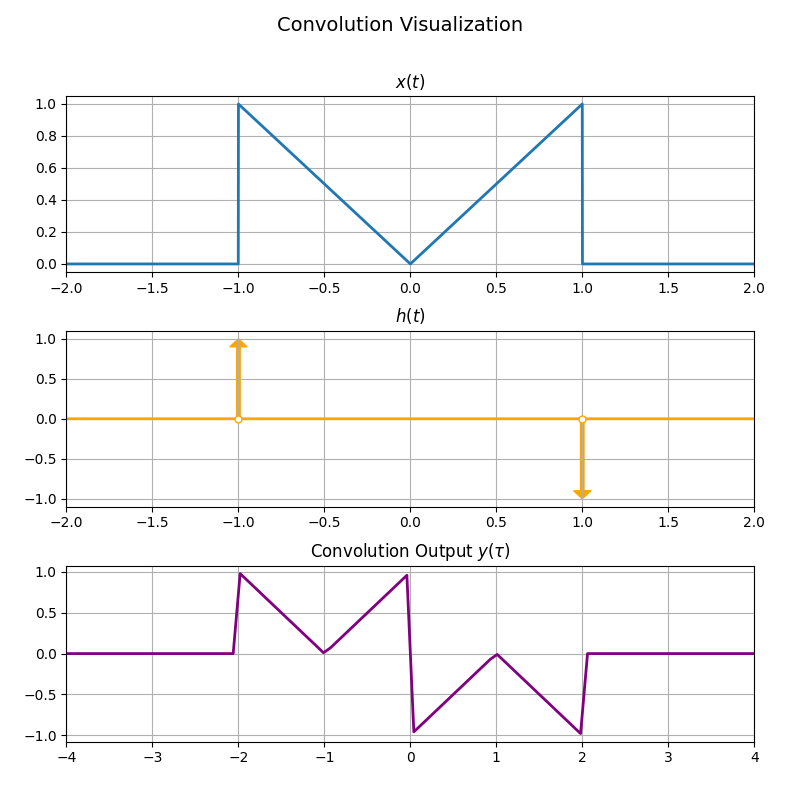
\includegraphics[width=0.75\textwidth]{images/problem_2_4_snapshot.png}
    \end{center}
\end{solution}
% ==================== %
% ================================================================================ %


% ================================================================================ %
%                                    Problem 03                                    %
% ================================================================================ %
\begin{problem}
Let \( f(t) \) and \( g(t) \) be given as follows:
\begin{center}
    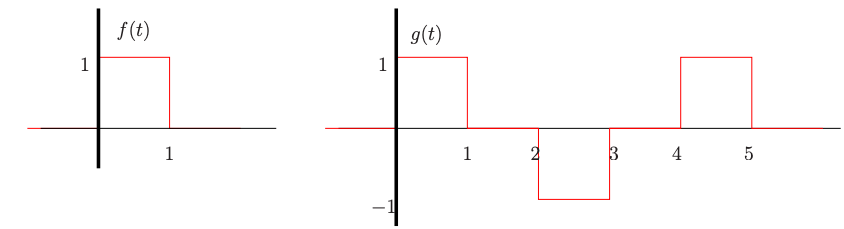
\includegraphics[width=0.8\textwidth]{images/problem_3_reference.png}
\end{center}
\end{problem}


% === Problem 3.1. === %
\begin{subproblems}[start=1]
    \item Sketch the function : \( x(t)$ = $f(t) * g(t) \)
\end{subproblems}

\begin{solution}
Using Python to visualize and compute the convolution graphically,
we can create an animation that demonstrates the convolution process step-by-step
as shown in the gif files in \href{https://github.com/patthadon-p/CEDT-2110203-CEM-II/blob/main/signal/homework-2/images/problem_3_1.gif}{Problem 3.1 Animation}.

\vspace{3mm}

\newpage
The plot of the signal is shown below:
\begin{center}
    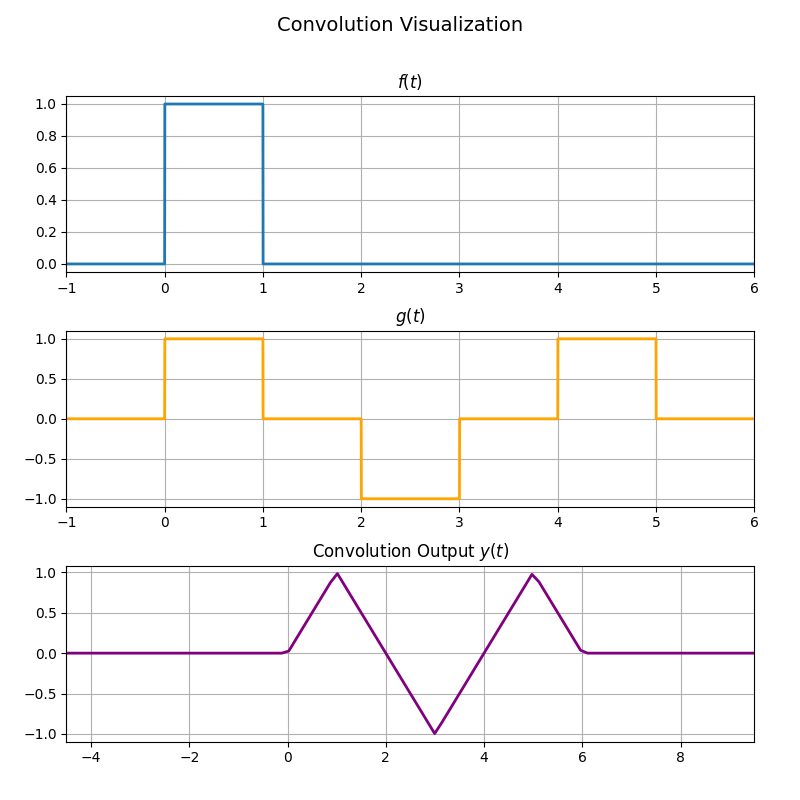
\includegraphics[width=0.75\textwidth]{images/problem_3_1_snapshot.png}
\end{center}
\end{solution}
% ==================== %


% === Problem 3.2. === %
\begin{subproblems}[start=2]
    \item Show that if \( a(t) = b(t) * c(t) \), then \( (Mb(t))*c(t) = Ma(t) \), for any real number \( M \) (hint: use the convolution integral formula)
\end{subproblems}

\begin{solution}
Given that \( a(t) = b(t) * c(t) \), we can express this using the convolution integral:
\[ a(t) = \int_{-\infty}^{\infty} b(\tau) c(t - \tau) \, d\tau \]

Now, we want to show that \( (Mb(t)) * c(t) = Ma(t) \). We start by writing the convolution of \( Mb(t) \) with \( c(t) \):
\[ (Mb(t)) * c(t) = \int_{-\infty}^{\infty} Mb(\tau) c(t - \tau) \, d\tau \]

Factoring out the constant \( M \) from the integral, we have:
\[ (Mb(t)) * c(t) = M \int_{-\infty}^{\infty} b(\tau) c(t - \tau) \, d\tau \]
\[ (Mb(t)) * c(t) = M a(t) \]

Thus, we have shown that:
\[ \boxed{(Mb(t)) * c(t) = Ma(t)} \]
\end{solution}
% ==================== %
% ================================================================================ %

\newpage

% ================================================================================ %
%                                    Problem 04                                    %
% ================================================================================ %
\begin{problem}
Find the convolution \( y[n] = h[n] * x[n] \) of the following signals:
\end{problem}

% === Problem 4.1. === %
\begin{tosubmit}
\begin{subproblems}[start=1]
    \item \( x[n] = \begin{cases} -1 , -5 \leq n \leq -1 \\ 1 , 0 \leq n \leq 4 \end{cases},\, h[n] = 2u[n] \)
\end{subproblems}

\par\noindent\submitsolution
To find the convolution \( y[n] = h[n] * x[n] \), we use the discrete convolution formula:
\[ y[n] = \sum_{k=-\infty}^{\infty} x[k] h[n - k] \]

Consider the value of \( y[n] \):
\begin{align*}
    y[n] &= \sum_{k=-\infty}^{\infty} x[k] h[n - k] \\
    &= \sum_{k=-5}^{-1} x[k] h[n - k] + \sum_{k=0}^{4} x[k] h[n - k] \\
    &= \sum_{k=-5}^{-1} (-1) \cdot 2u[n - k] + \sum_{k=0}^{4} (1) \cdot 2u[n - k] \\
    &= -2 \sqbracket{ \sum_{k=-5}^{-1} u[n - k] - \sum_{k=0}^{4} u[n - k] } \\
    y[n] &= -2 \sqbracket{ \sum_{j=n+1}^{n+5} u[j] - \sum_{j=n-4}^{n} u[j] } \\
\end{align*}

Calculating the convolution for different ranges of \( n \):
\begin{itemize}
    \item For \( -5 \leq n < 0 \):
    \begin{align*}
        y[n] &= -2 \sqbracket{ \sum_{j=n+1}^{n+5} u[j] - \sum_{j=n-4}^{n} u[j] } \\
        &= -2 \sqbracket{ n + 6  } \\
        y[n] &= -2n - 12
    \end{align*}
    \item For \( 0 \leq n < 5 \):
    \begin{align*}
        y[n] &= -2 \sqbracket{ \sum_{j=n+1}^{n+5} u[j] - \sum_{j=n-4}^{n} u[j] } \\
        &= -2 \sqbracket{ 5 - (n - 3) } \\
        y[n] &= 2n - 8
    \end{align*}
\end{itemize}

Thus, the final result of the convolution is:
\[ \boxed{
y[n] = \begin{cases}
-2n - 12 & -5 \leq n < 0 \\
2n - 8 & 0 \leq n < 5 \\
0 & \text{otherwise}
\end{cases}
} \]
\end{tosubmit}
% ==================== %

\newpage

% === Problem 4.2. === %
\begin{subproblems}[start=2]
    \item \( x[n] = u[n],\, h[n] = 1 \; ; 0 \leq n \leq 9 \)
\end{subproblems}

\begin{solution}
To find the convolution \( y[n] = h[n] * x[n] \), we use the discrete convolution formula:
\[ y[n] = \sum_{k=-\infty}^{\infty} x[k] h[n - k] \]

Consider the value of \( y[n] \):
\begin{align*}
    y[n] &= \sum_{k=-\infty}^{\infty} x[k] h[n - k] \\
    &= \sum_{k=0}^{\infty} u[k] \cdot h[n - k] \\
    &= \sum_{k=0}^{\infty} 1 \cdot h[n - k] \\
    y[n] &= \sum_{j=-\infty}^{n} h[j]
\end{align*}

Calculating the convolution for different ranges of \( n \):
\begin{itemize}
    \item For \( 0 \leq n < 9 \):
    \begin{align*}
        y[n] &= \sum_{j=-\infty}^{n} h[j] \\
        &= \sum_{j=0}^{n} 1 \\
        y[n] &= n + 1
    \end{align*}
    \item For \( n \geq 9 \):
    \begin{align*}
        y[n] &= \sum_{j=-\infty}^{n} h[j] \\
        &= \sum_{j=0}^{9} 1 \\
        y[n] &= 10
    \end{align*}
\end{itemize}

Thus, the final result of the convolution is:
\[ \boxed{
y[n] = \begin{cases}
n + 1 & 0 \leq n < 9 \\
10 & n \geq 9 \\
0 & \text{otherwise}
\end{cases}
} \]
\end{solution}
% ==================== %

\newpage

% === Problem 4.3. === %
\begin{tosubmit}    
\begin{subproblems}[start=3]
    \item \( x[n] = \paren{ \frac{1}{2} }^n u[n],\, h[n] = \delta[n] +\delta[n-1] +  \paren{ \frac{1}{3} }^n u[n] \)
\end{subproblems}

\par\noindent\submitsolution
To find the convolution \( y[n] = h[n] * x[n] \), we use the discrete convolution formula:
\[ y[n] = \sum_{k=-\infty}^{\infty} x[k] h[n - k] \]

Consider the value of \( y[n] \):
\begin{align*}
    y[n] &= \sum_{k=-\infty}^{\infty} x[k] h[n - k] \\
    &= \sum_{k=0}^{\infty} \paren{ \frac{1}{2} }^k u[k] \cdot \paren{ \delta[n - k] + \delta[n - k - 1] + \paren{ \frac{1}{3} }^{n - k} u[n - k] } \\
    y[n] &= \sum_{k=0}^{\infty} \paren{ \frac{1}{2} }^k \delta[n - k] + \sum_{k=0}^{\infty} \paren{ \frac{1}{2} }^k \delta[n - k - 1] + \sum_{k=0}^{\infty} \paren{ \frac{1}{2} }^k \paren{ \frac{1}{3} }^{n - k} u[n - k] \\
\end{align*}

Calculating the convolution for different ranges of \( n \):
\begin{itemize}
    \item For \( n \geq 0 \):
    \begin{align*}
        y[n] &= \sum_{k=0}^{\infty} \paren{ \frac{1}{2} }^k \delta[n - k] + \sum_{k=0}^{\infty} \paren{ \frac{1}{2} }^k \delta[n - k - 1] + \sum_{k=0}^{\infty} \paren{ \frac{1}{2} }^k \paren{ \frac{1}{3} }^{n - k} u[n - k] \\
        &= \paren{ \frac{1}{2} }^n + \paren{ \frac{1}{2} }^{n-1} + \sum_{k=0}^{n} \paren{ \frac{1}{2} }^k \paren{ \frac{1}{3} }^{n - k} \\
        &= \paren{ \frac{1}{2} }^n + 2 \paren{ \frac{1}{2} }^n + \paren{ \frac{1}{3} }^n \sum_{k=0}^{n} \paren{ \frac{3}{2} }^k \\
        &= 3 \paren{ \frac{1}{2} }^n + \paren{ \frac{1}{3} }^n \frac{1 - \paren{ \frac{3}{2} }^{n+1}}{1 - \frac{3}{2}} \\
        &= 3 \paren{ \frac{1}{2} }^n + \paren{ \frac{1}{3} }^n (-2)\paren{ 1 - \paren{ \frac{3}{2} }^{n+1}} \\
        &= 3 \paren{ \frac{1}{2} }^n + (-2) \paren{ \frac{1}{3} }^{n} + 3 \paren{ \frac{1}{2} }^{n} \\
        y[n] &= 6 \paren{ \frac{1}{2} }^n - 2 \paren{ \frac{1}{3} }^{n} \\
    \end{align*}
\end{itemize}

Thus, the final result of the convolution is:
\[ \boxed{
y[n] = \begin{cases}
6 \paren{ \frac{1}{2} }^n - 2 \paren{ \frac{1}{3} }^n & n \geq 0 \\
0 & \text{otherwise}
\end{cases}
} \]
\end{tosubmit}
% ==================== %

\newpage

% === Problem 4.4. === %
\begin{subproblems}[start=4]
    \item \( x[n] = \paren{ \frac{1}{3} }^n u[n],\, h[n] = \delta[n] + \paren{ \frac{1}{2} }^n u[n] \)
\end{subproblems}

\begin{solution}
To find the convolution \( y[n] = h[n] * x[n] \), we use the discrete convolution formula:
\[ y[n] = \sum_{k=-\infty}^{\infty} x[k] h[n - k] \]

Consider the value of \( y[n] \):
\begin{align*}
    y[n] &= \sum_{k=-\infty}^{\infty} x[k] h[n - k] \\
    &= \sum_{k=0}^{\infty} \paren{ \frac{1}{3} }^k u[k] \cdot \paren{ \delta[n - k] + \paren{ \frac{1}{2} }^{n - k} u[n - k] } \\
    y[n] &= \sum_{k=0}^{\infty} \paren{ \frac{1}{3} }^k \delta[n - k] + \sum_{k=0}^{\infty} \paren{ \frac{1}{3} }^k \paren{ \frac{1}{2} }^{n - k} u[n - k] \\
\end{align*}

Calculating the convolution for different ranges of \( n \):
\begin{itemize}
    \item For \( n \geq 0 \):
    \begin{align*}
        y[n] &= \sum_{k=0}^{\infty} \paren{ \frac{1}{3} }^k \delta[n - k] + \sum_{k=0}^{\infty} \paren{ \frac{1}{3} }^k \paren{ \frac{1}{2} }^{n - k} u[n - k] \\
        &= \paren{ \frac{1}{3} }^n + \sum_{k=0}^{n} \paren{ \frac{1}{3} }^k \paren{ \frac{1}{2} }^{n - k} \\
        &= \paren{ \frac{1}{3} }^n + \paren{ \frac{1}{2} }^n \sum_{k=0}^{n} \paren{ \frac{2}{3} }^k \\
        &= \paren{ \frac{1}{3} }^n + \paren{ \frac{1}{2} }^n \cdot \frac{1 - \paren{ \frac{2}{3} }^{n+1}}{1 - \frac{2}{3}} \\
        &= \paren{ \frac{1}{3} }^n + 3 \paren{ \frac{1}{2} }^n \sqbracket{ 1 - \paren{ \frac{2}{3} }^{n+1} } \\
        &= \paren{ \frac{1}{3} }^n + 3 \paren{ \frac{1}{2} }^n - 2 \paren{ \frac{1}{3} }^{n} \\
        y[n] &= 3 \paren{ \frac{1}{2} }^n - \paren{ \frac{1}{3} }^{n} \\
    \end{align*}
\end{itemize}

Thus, the final result of the convolution is:
\[ \boxed{
y[n] = \begin{cases}
3 \paren{ \frac{1}{2} }^n - \paren{ \frac{1}{3} }^n & n \geq 0 \\
0 & \text{otherwise}
\end{cases}
} \]
\end{solution}
% ==================== %
% ================================================================================ %

\newpage

% ================================================================================ %
%                                    Problem 05                                    %
% ================================================================================ %
\begin{problem}
    Find the convolution \( y[n] = h[n] * x[n] \) of the following signals
\end{problem}

% === Problem 5.1. === %
\begin{subproblems}[start=1]
    \item \( x[n] = \set{ 1, -\frac{1}{2}, \frac{1}{4}, -\frac{1}{8}, \frac{1}{16} },\, h[n] = \set{ 1, -1, 1, -1 } \)
\end{subproblems}

\begin{solution}
Using the tabular method to compute the convolution \( y[n] = h[n] * x[n] \):

\renewcommand{\arraystretch}{1.3}
\[
\begin{array}{c|ccc:ccccc:ccc||r}
n  & -3 & -2 & -1 & 0 & 1 & 2 & 3 & 4 & 5 & 6 & 7 & y[n] \\
\hline
x[n] &  &  &  & 1 & -\frac{1}{2} & \frac{1}{4} & -\frac{1}{8} & \frac{1}{16} &  &  &  &  \\
h[n] &  &  &  & 1 & -1 & 1 & -1 &  &  &  &  &  \\
\hline
h[0-n] & -1 & 1 & -1 & 1 &  &  &  &  &  &  &  & 1.0000 \\
h[1-n] &  & -1 & 1 & -1 & 1 &  &  &  &  &  &  & -1.5000 \\
h[2-n] &  &  & -1 & 1 & -1 & 1 &  &  &  &  &  & 1.7500 \\
h[3-n] &  &  &  & -1 & 1 & -1 & 1 &  &  &  &  & -1.8750 \\
h[4-n] &  &  &  &  & -1 & 1 & -1 & 1 &  &  &  & 0.9375 \\
h[5-n] &  &  &  &  &  & -1 & 1 & -1 & 1 &  &  & -0.4375 \\
h[6-n] &  &  &  &  &  &  & -1 & 1 & -1 & 1 &  & 0.1875 \\
h[7-n] &  &  &  &  &  &  &  & -1 & 1 & -1 & 1 & -0.0625 \\
\hline
\end{array}
\]

Thus, the final result of the convolution is:
\[ \boxed{ y[n] = \set{ 1, -1.5, 1.75, -1.875, 0.9375, -0.4375, 0.1875, -0.0625 } } \]
\end{solution}
% ==================== %


% === Problem 5.2. === %
\begin{subproblems}[start=2]
    \item \( x[n] = \set{ 1, 2, 3, 0, -1 },\, h[n] = \set{ 2, -1, 3, 1, -2 } \)
\end{subproblems}

\begin{solution}
Using the tabular method to compute the convolution \( y[n] = h[n] * x[n] \):

\renewcommand{\arraystretch}{1.3}
\[
\begin{array}{c|cccc:ccccc:cccc||r}
n  & -4 & -3 & -2 & -1 & 0 & 1 & 2 & 3 & 4 & 5 & 6 & 7 & 8 & y[n] \\
\hline
x[n] &  &  &  &  & 1 & 2 & 3 & 0 & -1 &  &  &  &  \\
h[n] &  &  &  &  & 2 & -1 & 3 & 1 & -2 &  &  &  &  \\
\hline
h[0-n] & -2 & 1 & 3 & -1 & 2 &  &  &  &  &  &  &  &  & 2 \\
h[1-n] &  & -2 & 1 & 3 & -1 & 2 &  &  &  &  &  &  &  & 3 \\
h[2-n] &  &  & -2 & 1 & 3 & -1 & 2 &  &  &  &  &  &  & 7 \\
h[3-n] &  &  &  & -2 & 1 & 3 & -1 & 2 &  &  &  &  &  & 4 \\
h[4-n] &  &  &  &  & -2 & 1 & 3 & -1 & 2 &  &  &  &  & 7 \\
h[5-n] &  &  &  &  &  & -2 & 1 & 3 & -1 & 2 &  &  &  & 0 \\
h[6-n] &  &  &  &  &  &  & -2 & 1 & 3 & -1 & 2 &  &  & -9 \\
h[7-n] &  &  &  &  &  &  &  & -2 & 1 & 3 & -1 & 2 &  & -1 \\
h[8-n] &  &  &  &  &  &  &  &  & -2 & 1 & 3 & -1 & 2 & 2 \\
\hline
\end{array}
\]

Thus, the final result of the convolution is:
\[ \boxed{ y[n] = \set{ 2, 3, 7, 4, 7, 0, -9, -1, 2 } } \]
\end{solution}
% ==================== %

\newpage

% === Problem 5.3. === %
\begin{subproblems}[start=3]
    \item \( x[n] = \set{ 3, \frac{1}{2}, -\frac{1}{4}, 1, 4 },\, h[n] = \set{ 2, -1, \frac{1}{2}, -\frac{1}{2} } \)
\end{subproblems}

\begin{solution}
Using the tabular method to compute the convolution \( y[n] = h[n] * x[n] \):

\renewcommand{\arraystretch}{1.3}
\[
\begin{array}{c|ccc:ccccc:ccc||r}
n  & -3 & -2 & -1 & 0 & 1 & 2 & 3 & 4 & 5 & 6 & 7 & y[n] \\
\hline
x[n] &  &  &  & 3 & \frac{1}{2} & -\frac{1}{4} & 1 & 4 &  &  &  &  \\
h[n] &  &  &  & 2 & -1 & \frac{1}{2} & -\frac{1}{2} &  &  &  &  &  \\
\hline
h[0-n] & -\frac{1}{2} & \frac{1}{2} & -1 & 2 &  &  &  &  &  &  &  & 6.000 \\
h[1-n] &  & -\frac{1}{2} & \frac{1}{2} & -1 & 2 &  &  &  &  &  &  & -2.000 \\
h[2-n] &  &  & -\frac{1}{2} & \frac{1}{2} & -1 & 2 &  &  &  &  &  & 0.500 \\
h[3-n] &  &  &  & -\frac{1}{2} & \frac{1}{2} & -1 & 2 &  &  &  &  & 1.000 \\
h[4-n] &  &  &  &  & -\frac{1}{2} & \frac{1}{2} & -1 & 2 &  &  &  & 6.625 \\
h[5-n] &  &  &  &  &  & -\frac{1}{2} & \frac{1}{2} & -1 & 2 &  &  & -3.375 \\
h[6-n] &  &  &  &  &  &  & -\frac{1}{2} & \frac{1}{2} & -1 & 2 &  & 1.500 \\
h[7-n] &  &  &  &  &  &  &  & -\frac{1}{2} & \frac{1}{2} & -1 & 2 & -2.000 \\
\hline
\end{array}
\]

Thus, the final result of the convolution is:
\[ \boxed{ y[n] = \set{ 6, -2, 0.5, 1, 6.625, -3.375, 1.5, -2 } } \]
\end{solution}
% ==================== %


% === Problem 5.4. === %
\begin{subproblems}[start=4]
    \item \( x[n] = \set{ -1, \frac{1}{2}, \frac{3}{4}, -\frac{1}{5}, 1 },\, h[n] = \set{ 1, 1, 1, 1, 1 } \)
\end{subproblems}

\begin{solution}
Using the tabular method to compute the convolution \( y[n] = h[n] * x[n] \):

\renewcommand{\arraystretch}{1.3}
\[
\begin{array}{c|cccc:ccccc:cccc||r}
n  & -4 & -3 & -2 & -1 & 0 & 1 & 2 & 3 & 4 & 5 & 6 & 7 & 8 & y[n] \\
\hline
x[n] &  &  &  &  & -1 & \frac{1}{2} & \frac{3}{4} & -\frac{1}{5} & 1 &  &  &  &  \\
h[n] &  &  &  &  & 1 & 1 & 1 & 1 & 1 &  &  &  &  \\
\hline
h[0-n] & 1 & 1 & 1 & 1 & 1 &  &  &  &  &  &  &  &  & -1.00 \\
h[1-n] &  & 1 & 1 & 1 & 1 & 1 &  &  &  &  &  &  &  & 0.50 \\
h[2-n] &  &  & 1 & 1 & 1 & 1 & 1 &  &  &  &  &  &  & 0.25 \\
h[3-n] &  &  &  & 1 & 1 & 1 & 1 & 1 &  &  &  &  &  & 0.05 \\
h[4-n] &  &  &  &  & 1 & 1 & 1 & 1 & 1 &  &  &  &  & 1.05 \\
h[5-n] &  &  &  &  &  & 1 & 1 & 1 & 1 & 1 &  &  &  & 2.05 \\
h[6-n] &  &  &  &  &  &  & 1 & 1 & 1 & 1 & 1 &  &  & 1.55 \\
h[7-n] &  &  &  &  &  &  &  & 1 & 1 & 1 & 1 & 1 &  & 0.80 \\
h[8-n] &  &  &  &  &  &  &  &  & 1 & 1 & 1 & 1 & 1 & 1.00 \\
\hline
\end{array}
\]

Thus, the final result of the convolution is:
\[ \boxed{ y[n] = \set{ -1, -0.5, 0.25, 0.05, 1.05, 2.05, 1.55, 0.8, 1 } } \]
\end{solution}
% ==================== %

\vspace{3mm}

\begin{center}
Note that all of the convolutions in Problem 5 are also available in the gif files in \href{https://github.com/patthadon-p/CEDT-2110203-CEM-II/tree/main/signal/homework-2/images}{this repository}.
\end{center}
% ================================================================================ %

\newpage

% ================================================================================ %
%                                    Problem 06                                    %
% ================================================================================ %
\begin{problem}
\end{problem}

% === Problem 6.1. === %
\begin{subproblems}[start=1]
    \item \textbf{Convolution 1-D:} \vspace{2mm}
    \par\noindent The following code creates a gaussian pulse and its self convolutions.
    Study and apply the convolution between signal \texttt{e} and another signal \texttt{e} with noise (\texttt{e\_noise}) and write the report to analyze the results.

    \begin{codingbox}
from scipy import signal

t = np.linspace(-1, 1, 2 * 100, endpoint=False)
i, q, e = signal.gausspulse(t, fc=5, retquad=True, retenv=True)
plt.plot(t, e, "--",label = "original signal")
plt.legend(loc="upper right")
plt.show()

conv_e = np.convolve(e,e,"same")
plt.plot(t, e, "--",label = "original signal")
plt.plot(t, conv_e, "--",label = "self conv signal")
plt.legend(loc="upper right")
plt.show()

e_noise = e + np.random.randn(len(e))*2.5
conv_e_noise = np.convolve(e, e_noise,"same")

# TODO : Apply the convolution between signal e and another signal e with noise (e_noise) and check the results
    \end{codingbox}

    \par\noindent \textbf{Results:} \par\noindent \vspace{3mm}

    1. Original Signal \texttt{e}:
    \begin{center}
        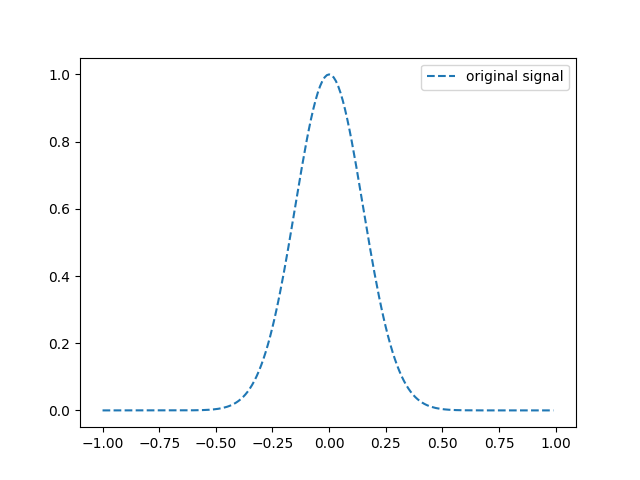
\includegraphics[width=0.75\textwidth]{images/problem_6_1_original_signal.png}
    \end{center}
    
    \newpage

    2. Convolution between signal \texttt{e} and signal \texttt{e}:
    \begin{center}
        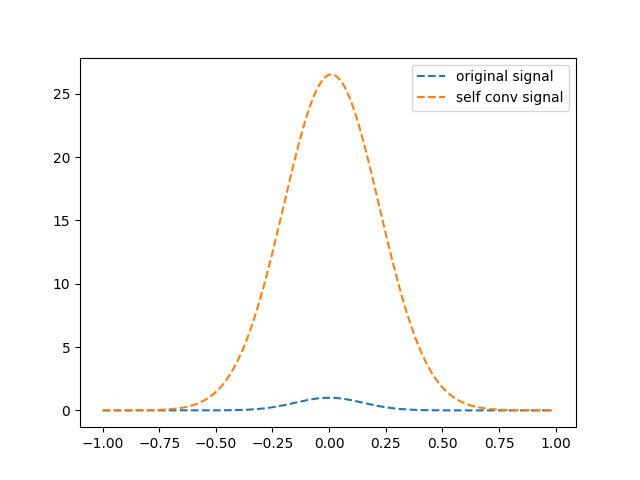
\includegraphics[width=0.75\textwidth]{images/problem_6_1_self_conv_signal.png}
    \end{center}
\end{subproblems}

\begin{solution}
To apply the convolution between the signal \( e \) and the noisy signal \( e\_noise \), we can use the following code snippet:

\begin{codingbox}
conv_e_noise = np.convolve(e, e_noise, "same")
plt.plot(t, e, "--", label="original signal")
plt.plot(t, conv_e_noise, "--", label="conv with noise signal")
plt.legend(loc="upper right")
plt.show()
\end{codingbox}

The result of the convolution between the original signal \( e \) and the noisy signal \( e\_noise \) is shown below:
\begin{center}
    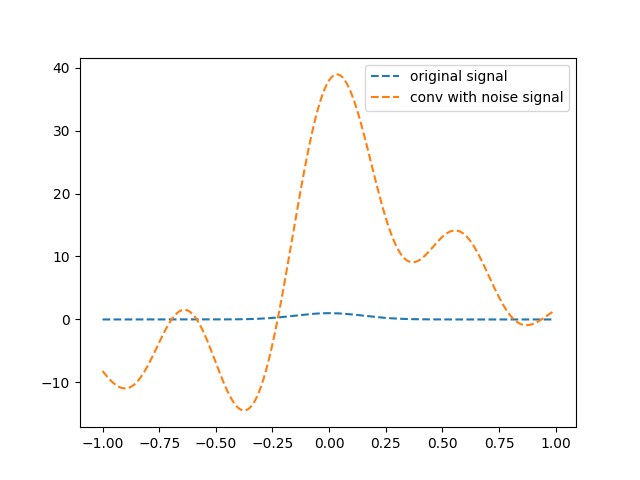
\includegraphics[width=0.75\textwidth]{images/problem_6_1_conv_with_noise_signal.png}
\end{center}
\end{solution}
% ==================== %

\newpage

% === Problem 6.2. === %
\begin{subproblems}[start=2]
    \item From the self convolution below, when increasing the number of self convolution (now is 8),
    what is noticeable from the final shape resulted from the convolution?

    \vspace{2mm}

    (\textbf{HINT 01:} Central limit theorem)

    \vspace{2mm}

    (\textbf{HINT 02:} What is Probability Density Function (PDF) of \( z \) if \( z = x + y \)? )

    \begin{codingbox}
from scipy.stats import uniform

x = np.linspace(-5,5, 1000)
plt.plot(x, uniform.pdf(x), "r-", lw=5, alpha=0.6, label="uniform pdf")
plt.show()

x = np.linspace(-15,15, 10000)
pdf_1 = uniform.pdf(x)
pdf_2 = uniform.pdf(x)

for i in range(8):
    pdf_2 = np.convolve(pdf_2,pdf_1, "same")

pdf_2 = pdf_2/np.max(pdf_2)
plt.plot(x, pdf_2,"r-", lw=5, alpha=0.6, label="conv uniform")
plt.show()
    \end{codingbox}

    \par\noindent \textbf{Results:} \par\noindent \vspace{3mm}
    1. Original Uniform PDF:
    \begin{center}
        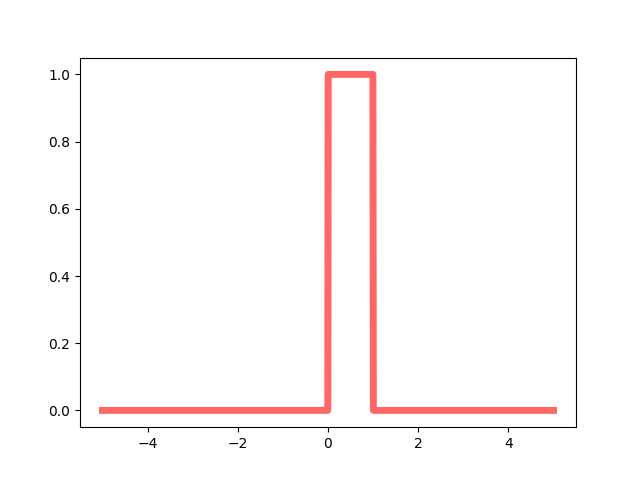
\includegraphics[width=0.75\textwidth]{images/problem_6_2_uniform_pdf.png}
    \end{center}

    \newpage

    2. Resulted PDF after 8 times of self convolution:
    \begin{center}
        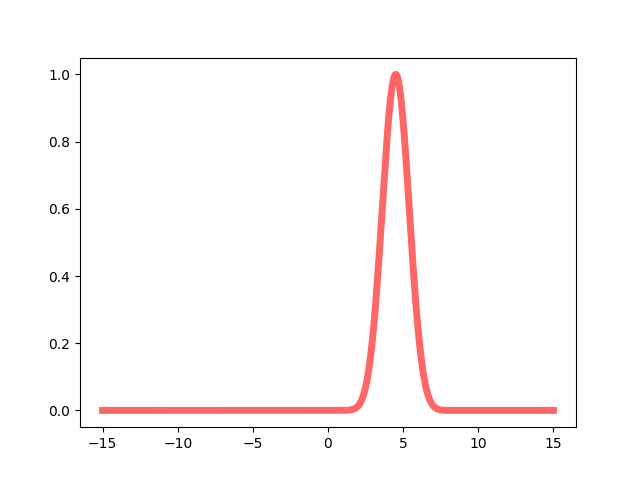
\includegraphics[width=0.75\textwidth]{images/problem_6_2_8_conv_uniform_pdf.png}
    \end{center}
\end{subproblems}

\begin{solution}
Firstly, we create a function to compute the PDF of a uniform distribution after specified number of self-convolutions. The code snippet is as follows:
\begin{codingbox}
def plot_uniform_convolution(ax, num_convolutions=1):
    x = np.linspace(-15, 15, 10000)
    pdf = uniform.pdf(x)

    conv_pdf = pdf.copy()
    for _ in range(num_convolutions):
        conv_pdf = np.convolve(conv_pdf, pdf, mode="same")

    conv_pdf = conv_pdf / np.max(conv_pdf)

    ax.plot(x, conv_pdf, "r-", lw=3, alpha=0.7, label=f"{num_convolutions} convolutions")
    ax.set_title(f"Uniform PDF convolved {num_convolutions} times")
    ax.set_xlabel("x")
    ax.set_ylabel("Normalized PDF")
    ax.legend()
    ax.grid(True)

    # Automatically adjust x-limits based on significant values
    threshold = 1e-4
    significant_indices = np.where(conv_pdf > threshold)[0]
    ax.set_xlim(x[significant_indices[0]], x[significant_indices[-1]])
\end{codingbox}

\newpage

Then, we can visualize the effect of multiple self-convolutions on the uniform PDF.
\begin{codingbox}
np.random.seed(1)  # For reproducibility

Ns = [1, 2, 4, 8, 12, 16]

# Create a 3x2 subplot grid
fig, axes = plt.subplots(3, 2, figsize=(8, 8))
axes = axes.flatten()  # Flatten to make indexing easier

for i, N in enumerate(Ns):
    plot_uniform_convolution(axes[i], N)
    
plt.tight_layout()
plt.savefig("../images/problem_6_2_comparation.png", dpi=600, bbox_inches="tight")
plt.show()
\end{codingbox}

The final shape resulted from the convolution approaches a Gaussian distribution as the number of self-convolutions increases.
This is a direct consequence of the \textbf{Central Limit Theorem},
which states that \textbf{the sum of a large number of independent random variables},
regardless of their original distribution, will tend to follow a \textbf{normal (Gaussian) distribution}.

\begin{center}
    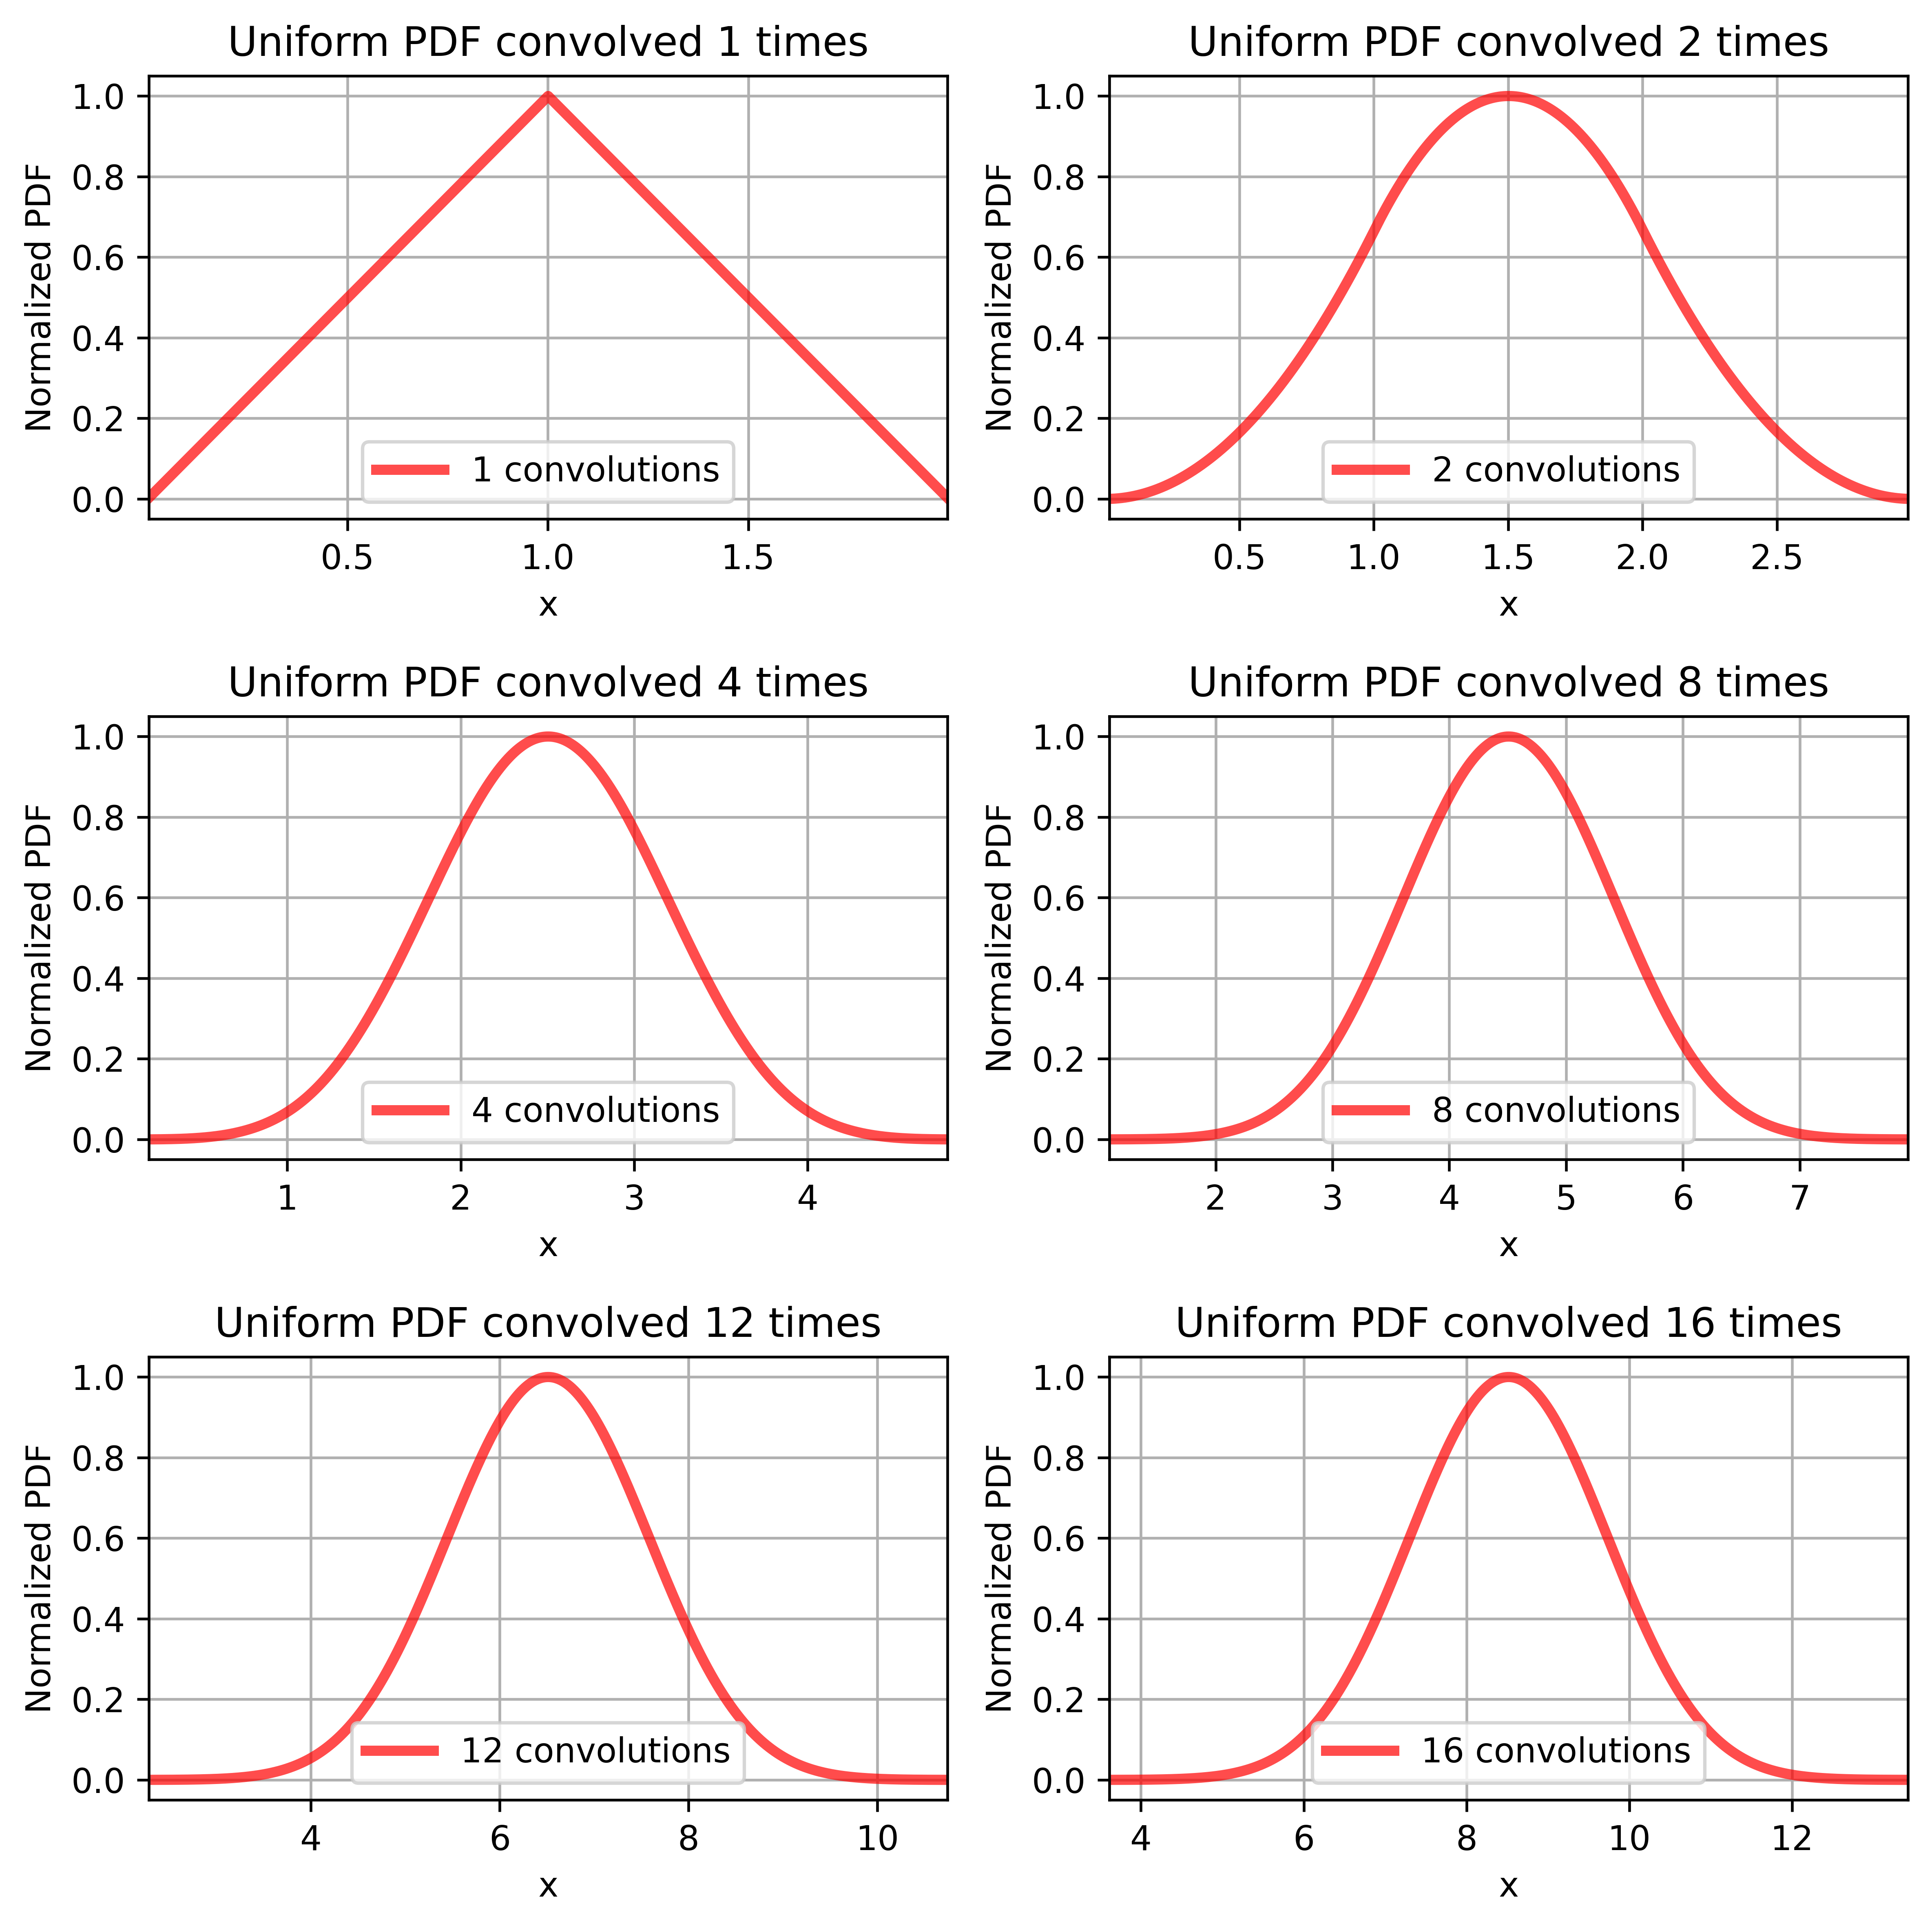
\includegraphics[width=0.75\textwidth]{images/problem_6_2_comparation.png}
\end{center}
\end{solution}
% ==================== %
% ================================================================================ %

\newpage

% ================================================================================ %
%                                    Problem 07                                    %
% ================================================================================ %
\begin{problem}
\textbf{2D (image) signal convolution:}

\vspace{2mm}

\par\noindent The following code show the 2D signal (image \( f(x, y) \)) and a kernel (diag\_line).
Study the convolution of the kernel and the image. Apply with \texttt{"circuits.png"} image and analyze the results.

\vspace{2mm}

\par\noindent\textbf{TODO :} Apply diag\_line to the \texttt{"circuits.png"} image and analyse the results

\begin{codingbox}
import cv2

image_path = "hamtaro0.jpg"

diag_line = np.array([[ 2, -1, -1],
                    [-1, 2, -1],
                    [-1, -1, 2]])

ham = cv2.imread(image_path, 0)
plt.figure(figsize=(10, 10))
plt.imshow(ham, cmap="gray")
plt.show()

grad = signal.convolve2d(ham, diag_line, boundary="symm", mode="same")
plt.figure(figsize=(10, 10))
plt.imshow(grad, cmap="gray")
plt.show()

# TODO : Apply diag_line to the "circuits.png" image and analyse the results
\end{codingbox}

\par\noindent \textbf{Results:} \par\noindent \vspace{3mm}
\begin{center}
    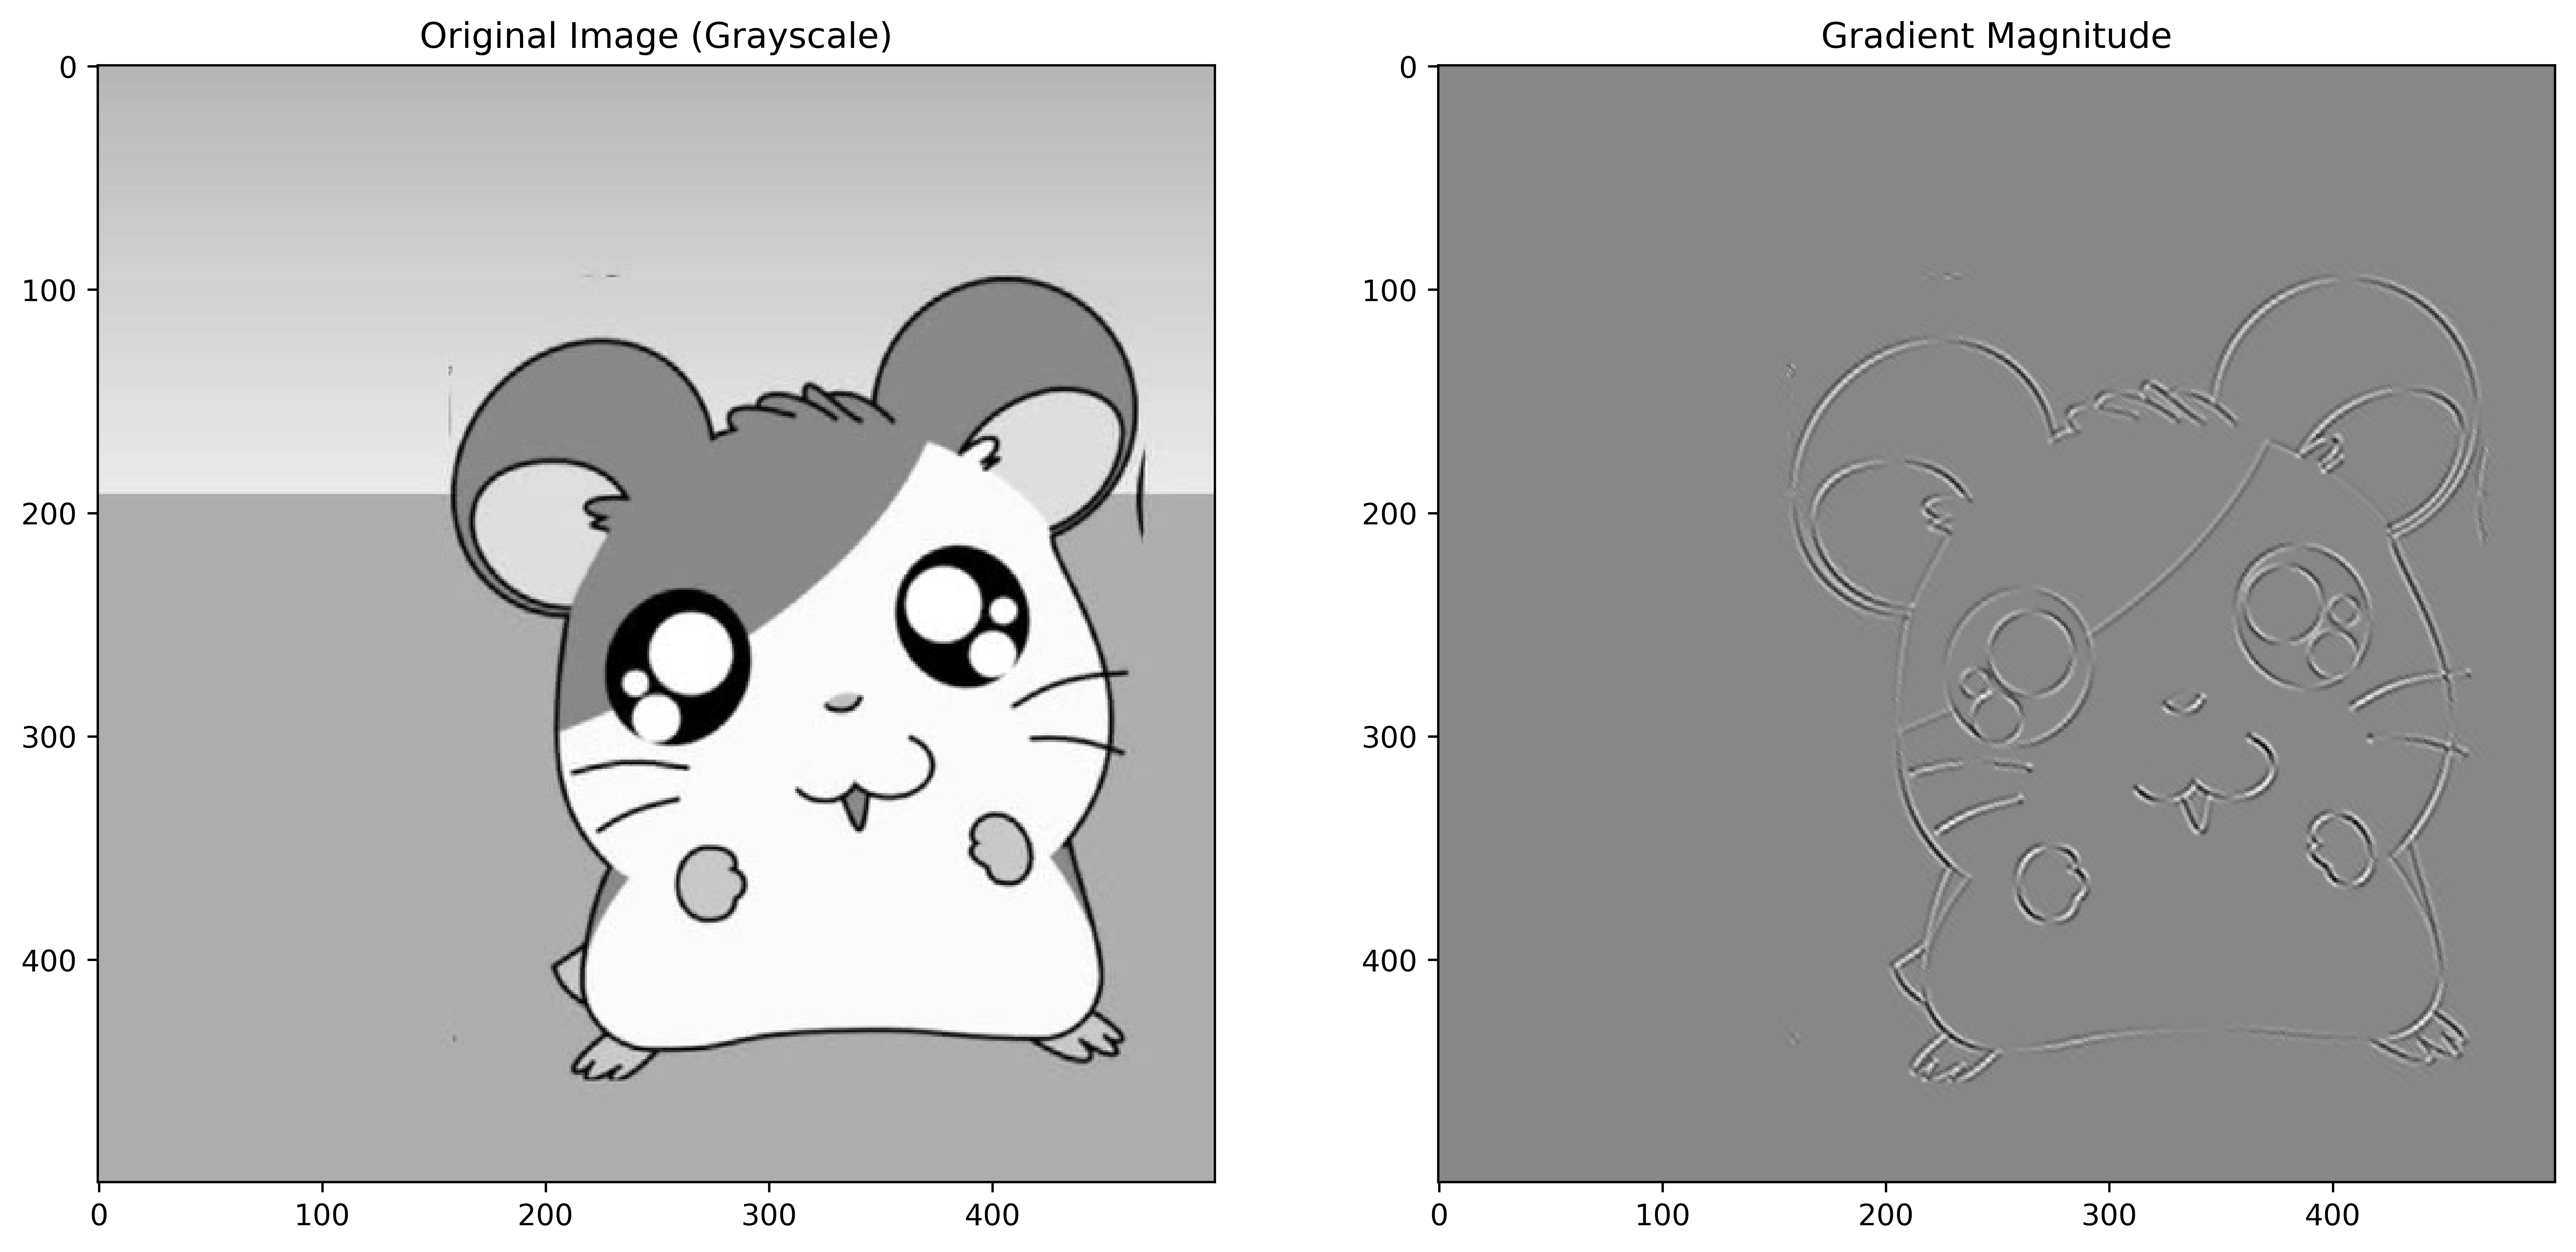
\includegraphics[width=0.75\textwidth]{images/problem_7_hamtaro_gradient.png}
\end{center}
\end{problem}

\newpage

\begin{solution}
To apply the convolution of the kernel \texttt{diag\_line} to the image \texttt{"circuits.png"}, we can use the following code snippet:

\begin{codingbox}
image_path = "../images/problem_7_circuits.png"

diag_line = np.array([[ 2, -1, -1],
                    [-1, 2, -1],
                    [-1, -1, 2]])

circuits = cv2.imread(image_path, 0)
plt.figure(figsize=(10, 10))
plt.imshow(circuits, cmap="gray")
plt.show()

grad = signal.convolve2d(circuits, diag_line, boundary="symm", mode="same")
plt.figure(figsize=(10, 10))
plt.imshow(grad, cmap="gray")
plt.show()
\end{codingbox}

The result of the convolution between the image \texttt{"circuits.png"} and the kernel \texttt{diag\_line} is shown below:
\begin{center}
    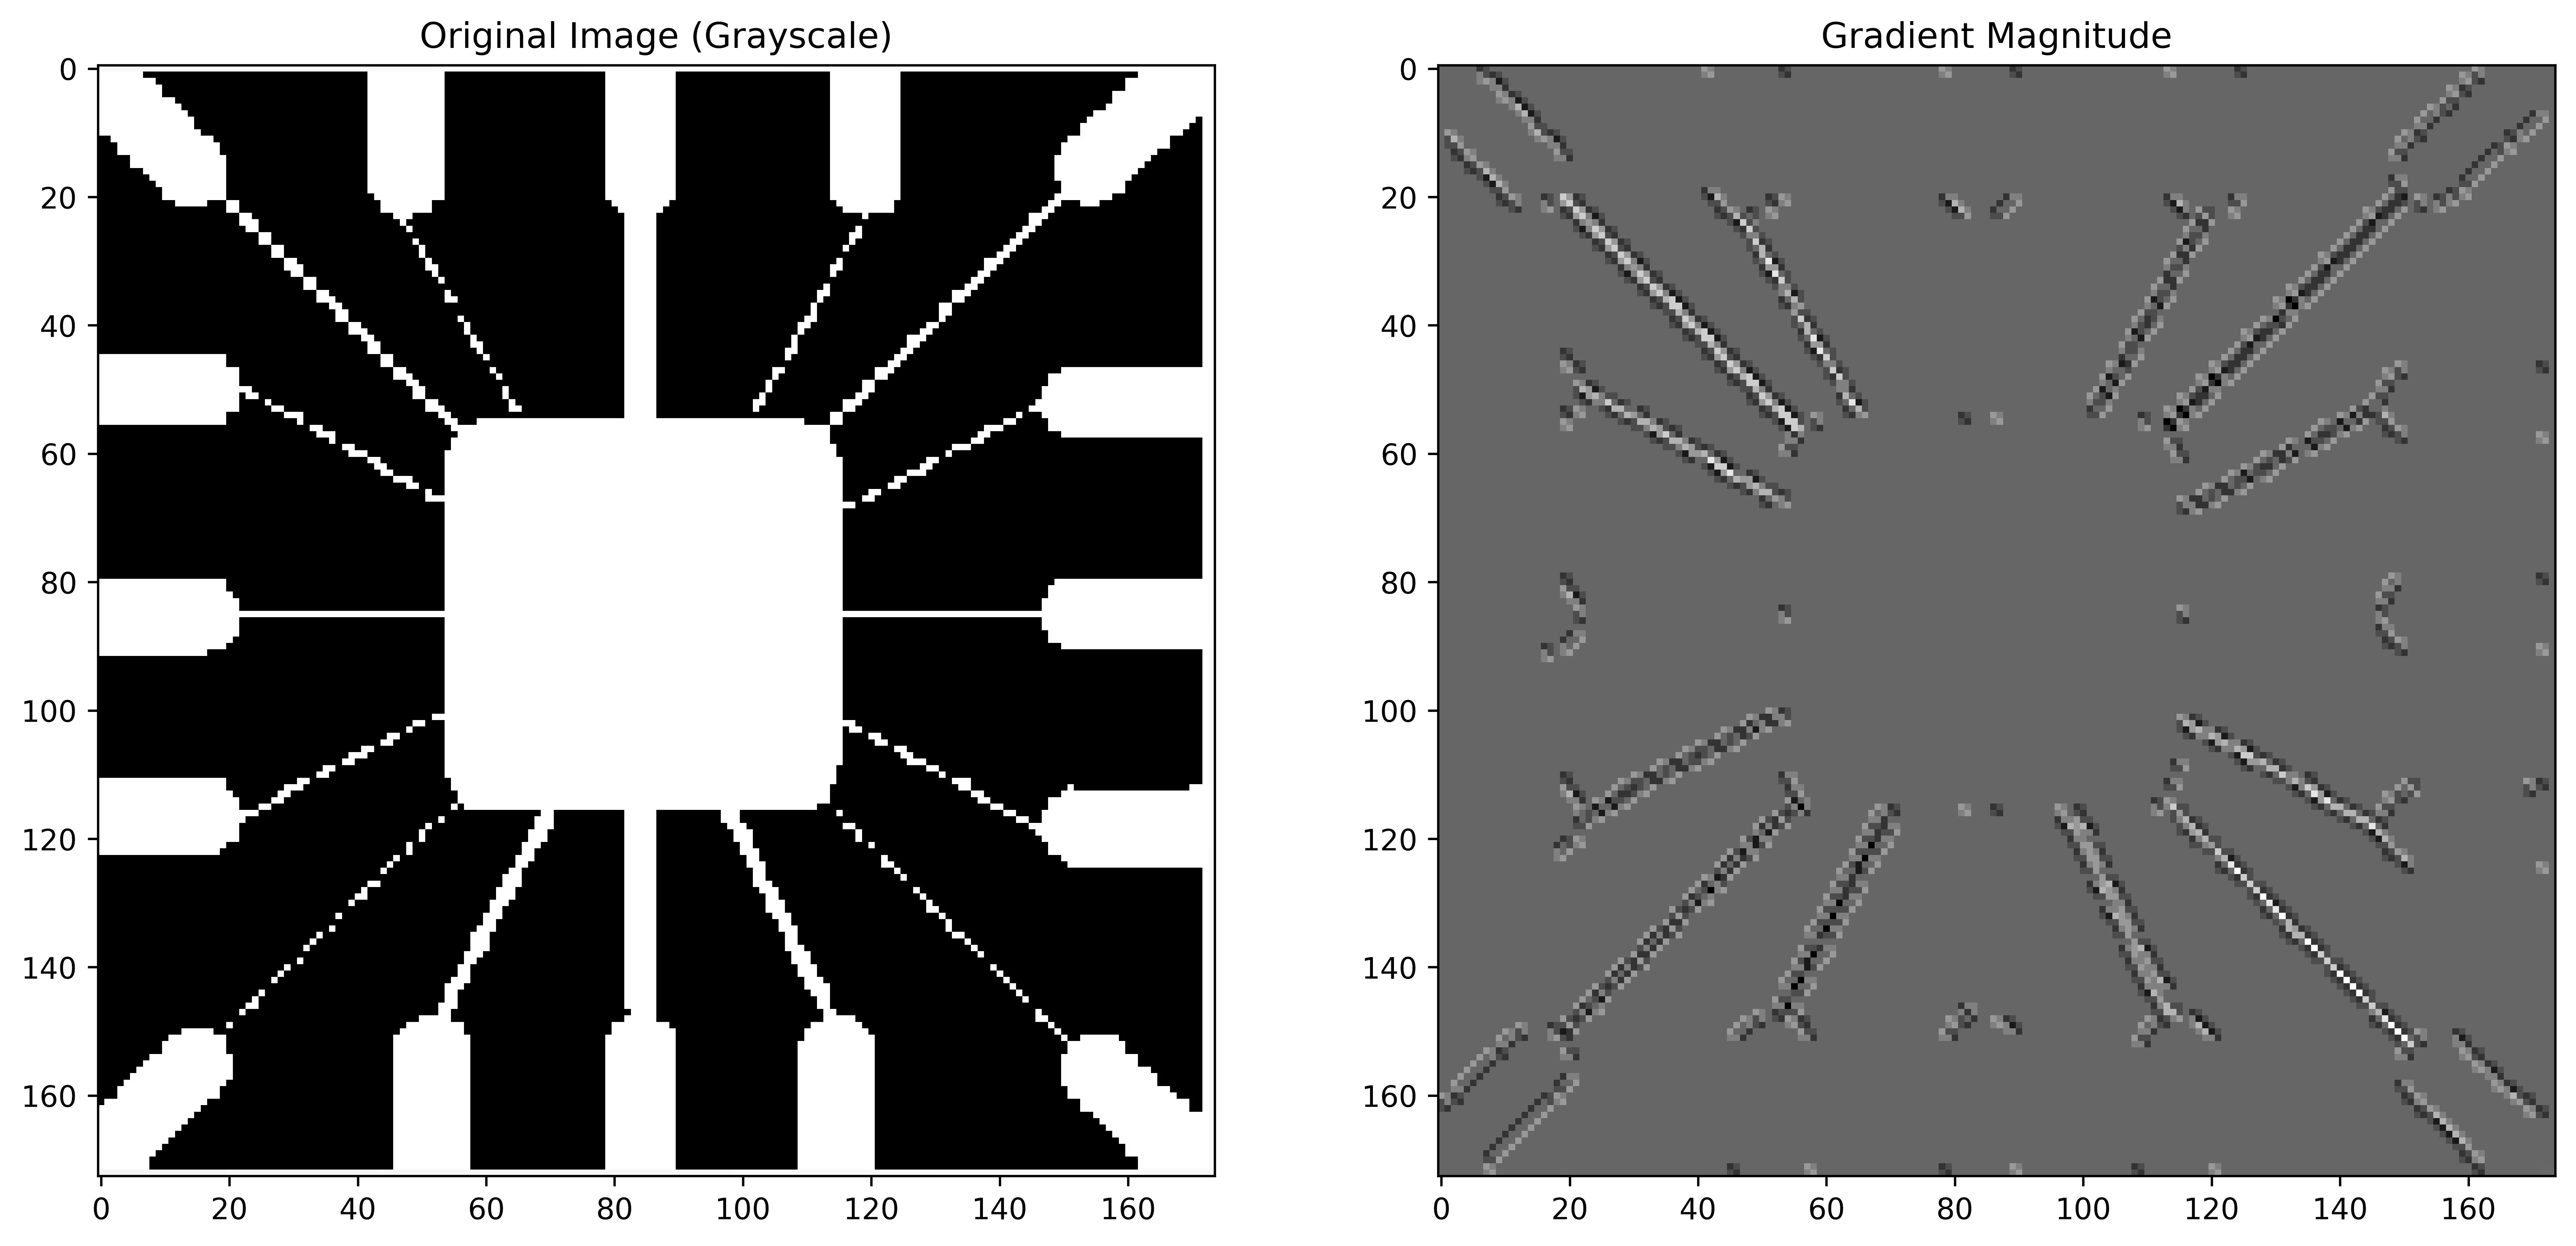
\includegraphics[width=0.75\textwidth]{images/problem_7_circuits_gradient.png}
\end{center}
\end{solution}
% ================================================================================ %

\newpage

% ================================================================================ %
%                                    Problem 08                                    %
% ================================================================================ %
\begin{problem}
Are the following systems linear or time invariant?
\end{problem}

% === Problem 8.1. === %
\begin{subproblems}[start=1]
    \item \( x(t) \rightarrow \) \textbf{System(a)} \( \rightarrow 7x(t-1) \)
\end{subproblems}

\begin{solution}
\vspace{2mm}

\par\noindent\textbf{1. Check for linearity:}
Let \( x_1(t) \) and \( x_2(t) \) be two input signals, consider,
\begin{align*}
S\{ a x_1(t) + b x_2(t) \} &= 7 [ a x_1(t-1) + b x_2(t-1) ] \\
&= 7 a x_1(t-1) + 7 b x_2(t-1) \\
&= a [ 7 x_1(t-1) ] + b [ 7 x_2(t-1) ] \\
S\{ a x_1(t) + b x_2(t) \} &= a S\{ x_1(t) \} + b S\{ x_2(t) \}
\end{align*}

Since both sides are equal, the system is linear.

\vspace{2mm}

\par\noindent\textbf{2. Check for time invariance:}
Let \( x(t) \) be an input signal and \( t_0 \) be a time shift, consider,
\begin{align*}
S\{ x(t - t_0) \} &= 7 x((t - t_0) - 1) \\
&= 7 x(t - t_0 - 1) \\
&= 7 x((t - 1) - t_0) \\
\implies S\{ x(t - t_0) \} &= y(t - t_0)
\end{align*}

Since both sides are equal, the system is time-invariant.

Therefore, the system \( S\{ x(t) \} = 7 x(t-1) \) is \( \boxed{\text{both linear and time-invariant}} \).
\end{solution}
% ==================== %


% === Problem 8.2. === %
\begin{subproblems}[start=2]
    \item \( x(t) \rightarrow \) \textbf{System(b)} \( \rightarrow \cos(2x(t)) \)
\end{subproblems}

\begin{solution}
\vspace{2mm}

\par\noindent\textbf{1. Check for linearity:}
Let \( x_1(t) \) and \( x_2(t) \) be two input signals, consider,
\begin{align*}
    \cos(2 [ a x_1(t) + b x_2(t) ]) &\neq a [ \cos(2 x_1(t)) ] + b [ \cos(2 x_2(t)) ] \\
    \implies S\{ a x_1(t) + b x_2(t) \} &= a S\{ x_1(t) \} + b S\{ x_2(t) \}
\end{align*}

Since both sides are not equal, the system is non-linear.

\vspace{2mm}

\par\noindent\textbf{2. Check for time invariance:}
Let \( x(t) \) be an input signal and \( t_0 \) be a time shift, consider,
\begin{align*}
S\{ x(t - t_0) \} &= \cos(2 [ x(t - t_0) ]) \\
&= \cos(2 x(t - t_0)) \\
\implies S\{ x(t - t_0) \} &= y(t - t_0)
\end{align*}

Since both sides are equal, the system is time-invariant.

Therefore, the system \( S\{ x(t) \} = \cos(2x(t)) \) is \( \boxed{\text{non-linear but time-invariant}} \).
\end{solution}
% ==================== %

\newpage

% === Problem 8.3. === %
\begin{subproblems}[start=3]
    \item \( x(t) \rightarrow \) \textbf{System(c)} \( \rightarrow t \)
\end{subproblems}

\begin{solution}
\vspace{2mm}

\par\noindent\textbf{1. Check for linearity:}
Let \( x_1(t) \) and \( x_2(t) \) be two input signals, consider,
\begin{align*}
t &\neq (a + b)t \\
&= a \cdot t + b \cdot t \\
\implies S\{ a x_1(t) + b x_2(t) \} &\neq a S\{ x_1(t) \} + b S\{ x_2(t) \}
\end{align*}

Since both sides are not equal, the system is non-linear.

\vspace{2mm}

\par\noindent\textbf{2. Check for time invariance:}
Let \( x(t) \) be an input signal and \( t_0 \) be a time shift, consider,
\begin{align*}
t &\neq t - t_0 \\
\implies S\{ x(t - t_0) \} &\neq y(t - t_0)
\end{align*}

Since both sides are not equal, the system is time-variant.

Therefore, the system \( S\{ x(t) \} = t \) is \( \boxed{\text{both non-linear and time-variant}} \).
\end{solution}
% ==================== %


% === Problem 8.4. === %
\begin{subproblems}[start=4]
    \item \( x(t) \rightarrow \) \textbf{System(d)} \( \rightarrow x(t)+t \)
\end{subproblems}

\begin{solution}
\vspace{2mm}

\par\noindent\textbf{1. Check for linearity:}
Let \( x_1(t) \) and \( x_2(t) \) be two input signals, consider,
\begin{align*}
a x_1(t) + b x_2(t) + t &\neq a [ x_1(t) + t ] + b [ x_2(t) + t ] \\
\implies S\{ a x_1(t) + b x_2(t) \} &\neq a S\{ x_1(t) \} + b S\{ x_2(t) \}
\end{align*}

Since both sides are not equal, the system is non-linear.

\vspace{2mm}

\par\noindent\textbf{2. Check for time invariance:}
Let \( x(t) \) be an input signal and \( t_0 \) be a time shift, consider,
\begin{align*}
x(t - t_0) + t &\neq x(t - t_0) + t - t_0 \\
\implies S\{ x(t - t_0) \} &\neq y(t - t_0)
\end{align*}

Since both sides are not equal, the system is time-variant.

Therefore, the system \( S\{ x(t) \} = x(t) + t \) is \( \boxed{\text{both non-linear and time-variant}} \).
\end{solution}
% ==================== %
% ================================================================================ %

\end{document}